\documentclass{article}
\usepackage[spanish]{babel}
\usepackage{graphicx}
\usepackage{xcolor}
\usepackage[utf8]{inputenc}
\usepackage{fancyhdr}
\usepackage{lastpage}
\usepackage{enumitem}
\usepackage{listings}
\usepackage{float}
\usepackage{verbatim}

\pagestyle{fancy}
\fancyhf{}
\rfoot{Page \thepage\hspace{1pt} de~\pageref{LastPage}}

\title{Práctica Web Crawler}
\author{Guillermo López García}

\begin{document}
\maketitle

\textbf{Ejercicios.}
\begin{enumerate}
    \item He obtenido los siguientes resultados:
        \begin{figure}[H]
        \centering
        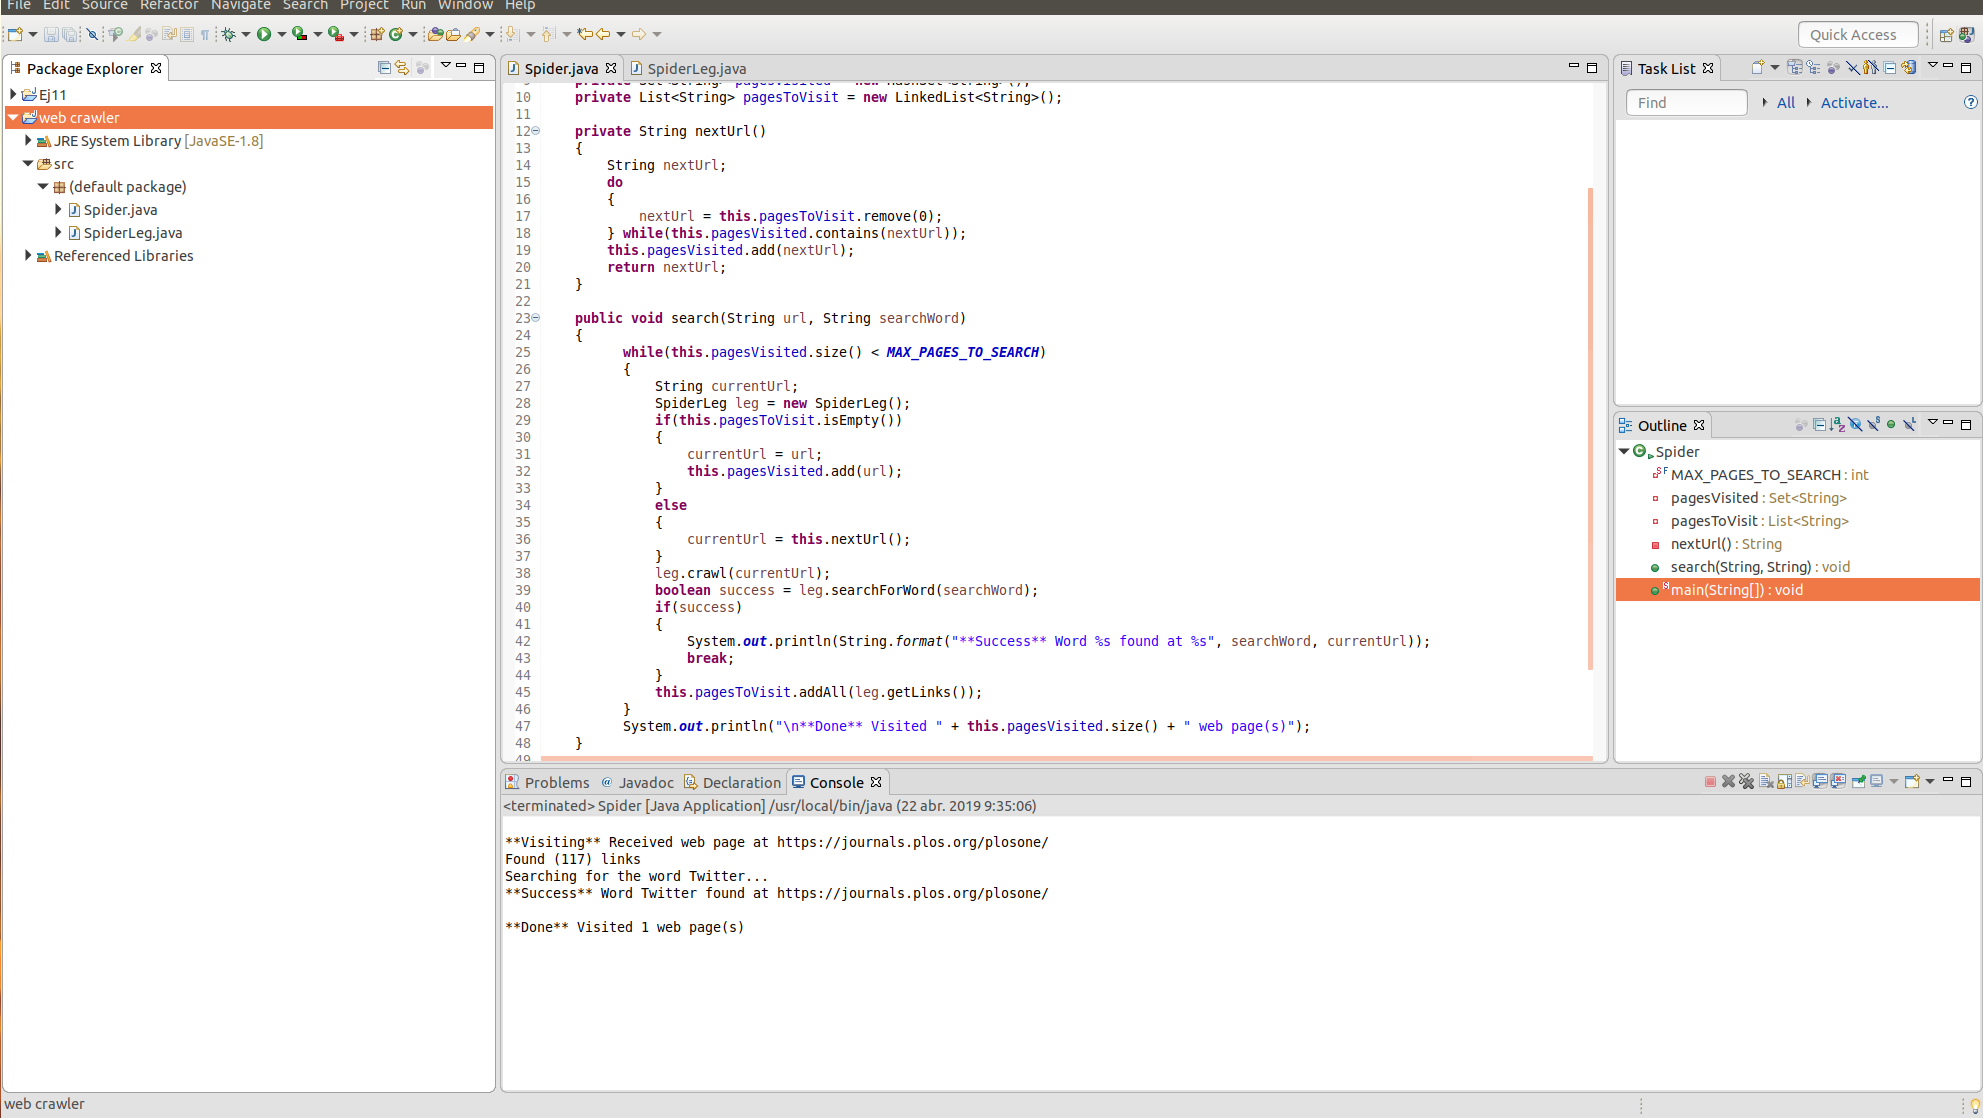
\includegraphics[width=0.7\linewidth]{./ej1}
        \caption{Ejercicio 1.}
        \end{figure}
    
    \item He obtenido los siguientes resultados:
        \begin{figure}[H]
        \centering
        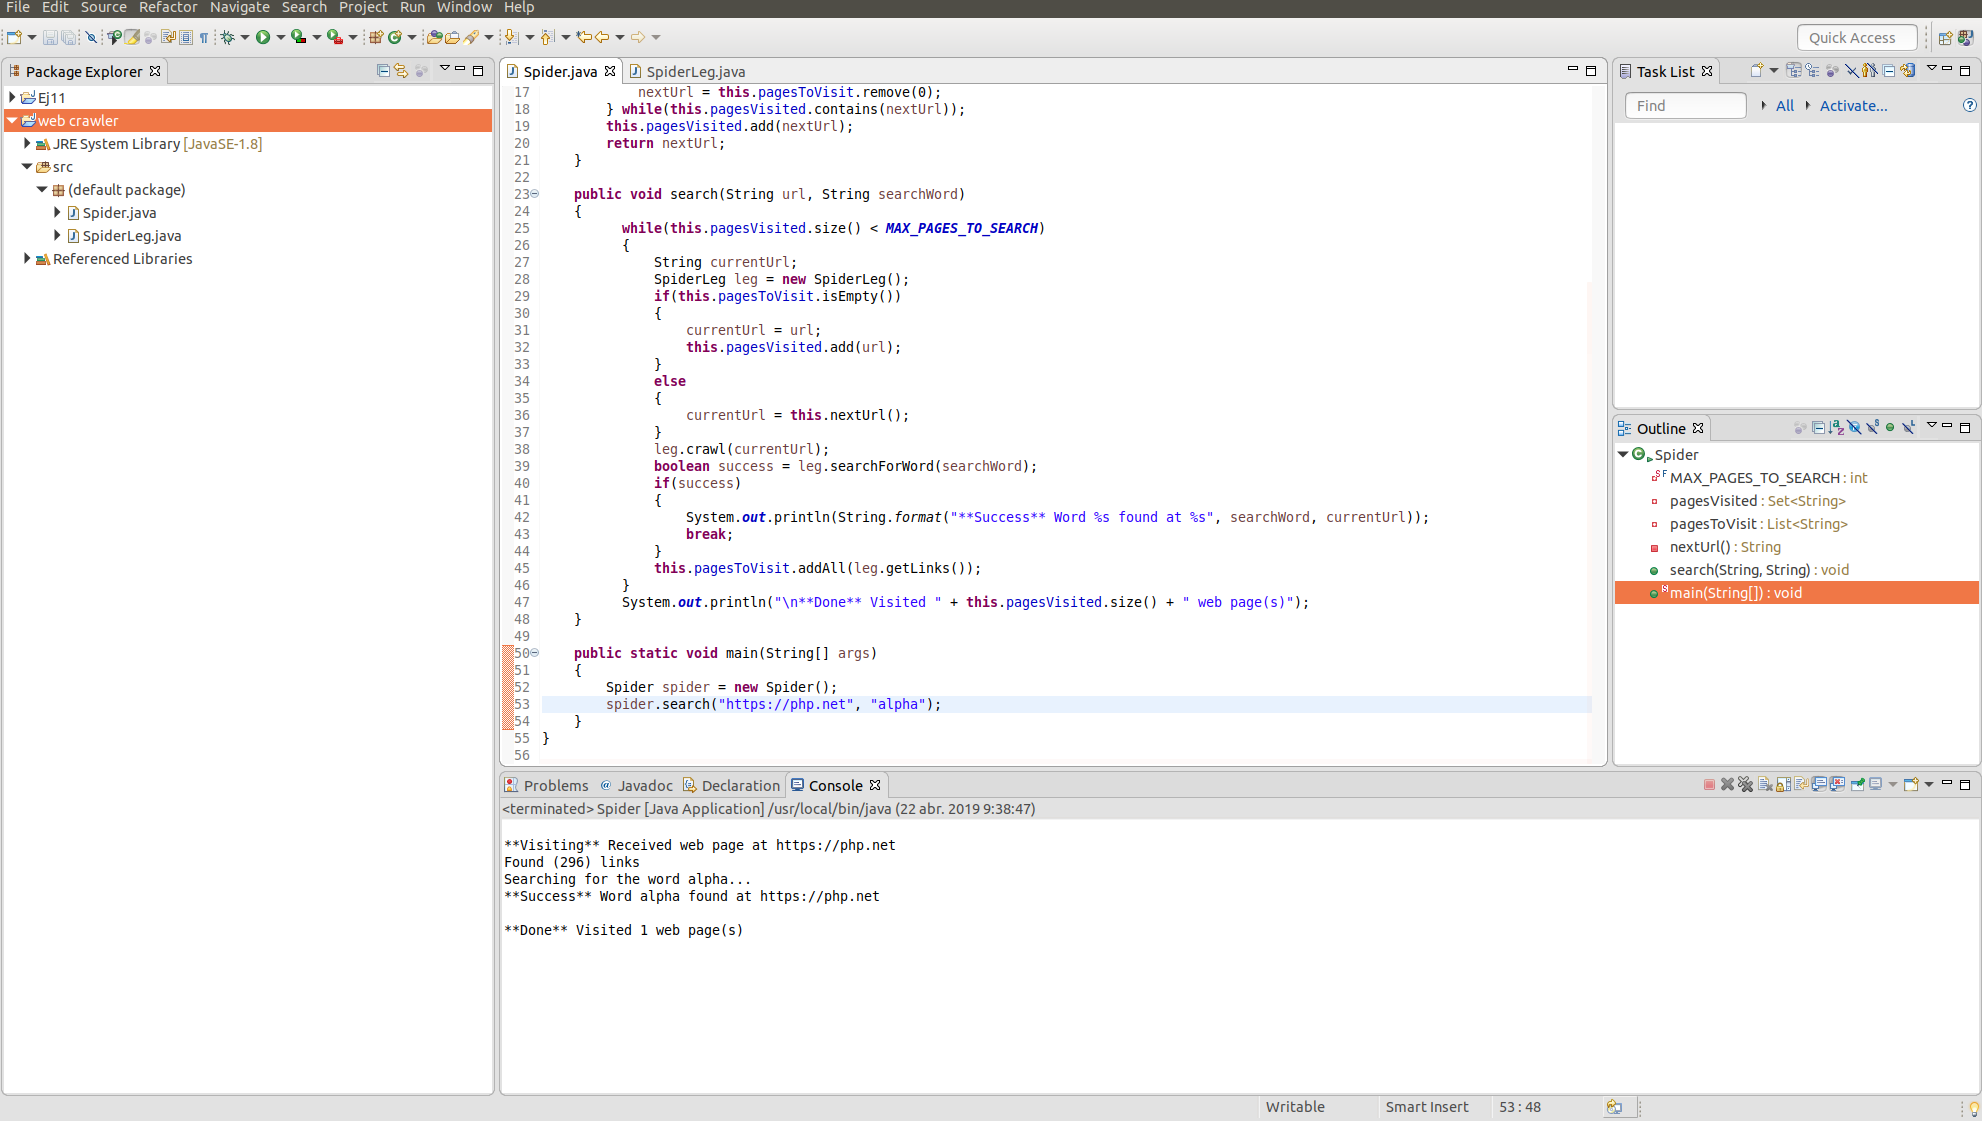
\includegraphics[width=0.7\linewidth]{./ej2}
        \caption{Ejercicio 2.}
        \end{figure}
        
    \item He aquí el código creado para resolver dicho problema:
        \lstset{
          language=Java,
          texcl=true,
          basicstyle=\ttfamily,
          columns=fullflexible,
          frame=single,
          breaklines=true,
          postbreak=\mbox{\textcolor{red}{$\hookrightarrow$}\space},
        }
        \lstinputlisting[]{Spider.java}
        
        \lstset{
          language=Java,
          texcl=true,
          basicstyle=\ttfamily,
          columns=fullflexible,
          frame=single,
          breaklines=true,
          postbreak=\mbox{\textcolor{red}{$\hookrightarrow$}\space},
        }
        \lstinputlisting[]{SpiderLeg.java}
\end{enumerate}

\end{document}
